\documentclass[t,aspectratio=169]{beamer}
%\usetheme{Berkeley}
\usepackage{graphicx}
\usepackage{amsmath}
\usepackage[american]{circuitikz}

\title{Clase 16}
\subtitle{Efecto Early}
\author{Dr.-Ing. Juan José Montero Rodríguez}
\subject{Elementos Activos}
\institute{Escuela de Ingeniería Electrónica}
\date{Semestre II-2023}

\begin{document}

\begin{frame}{}
\maketitle
\end{frame}



\begin{frame}{Efecto Early}

\begin{itemize}
    \item El transistor de la figura (a) está en Activa Directa, y la tensión $V_C > V_B$.
    \item Si se aumenta la tensión $V_C$ en la figura (b), el ancho de la región de agotamiento B-C aumenta.
\end{itemize}

\begin{figure}[H]
    \centering
    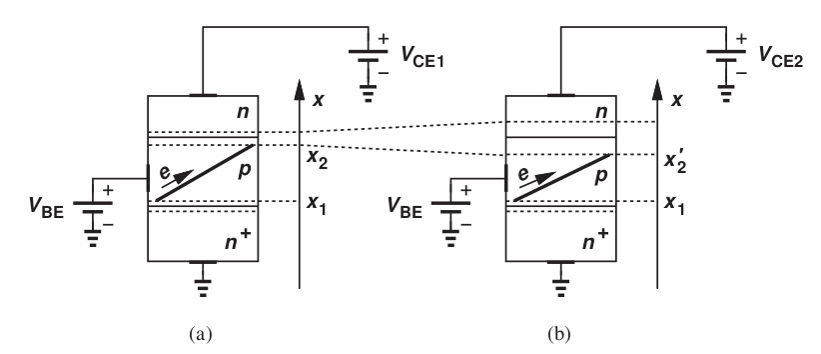
\includegraphics[width=0.7\textwidth]{figuras/efecto_early_sentido_fisico.png}
\end{figure}

\begin{itemize}
    \item El ancho de la base en (b) es más corto: $W_B = x_2' - x_1$
\end{itemize}

\end{frame}


\begin{frame}{Corriente de colector con efecto Early}

El ancho de la base depende de la tensión aplicada entre el colector y emisor.


\begin{columns}
\begin{column}{0.4\textwidth}

\begin{figure}[H]
    \centering
    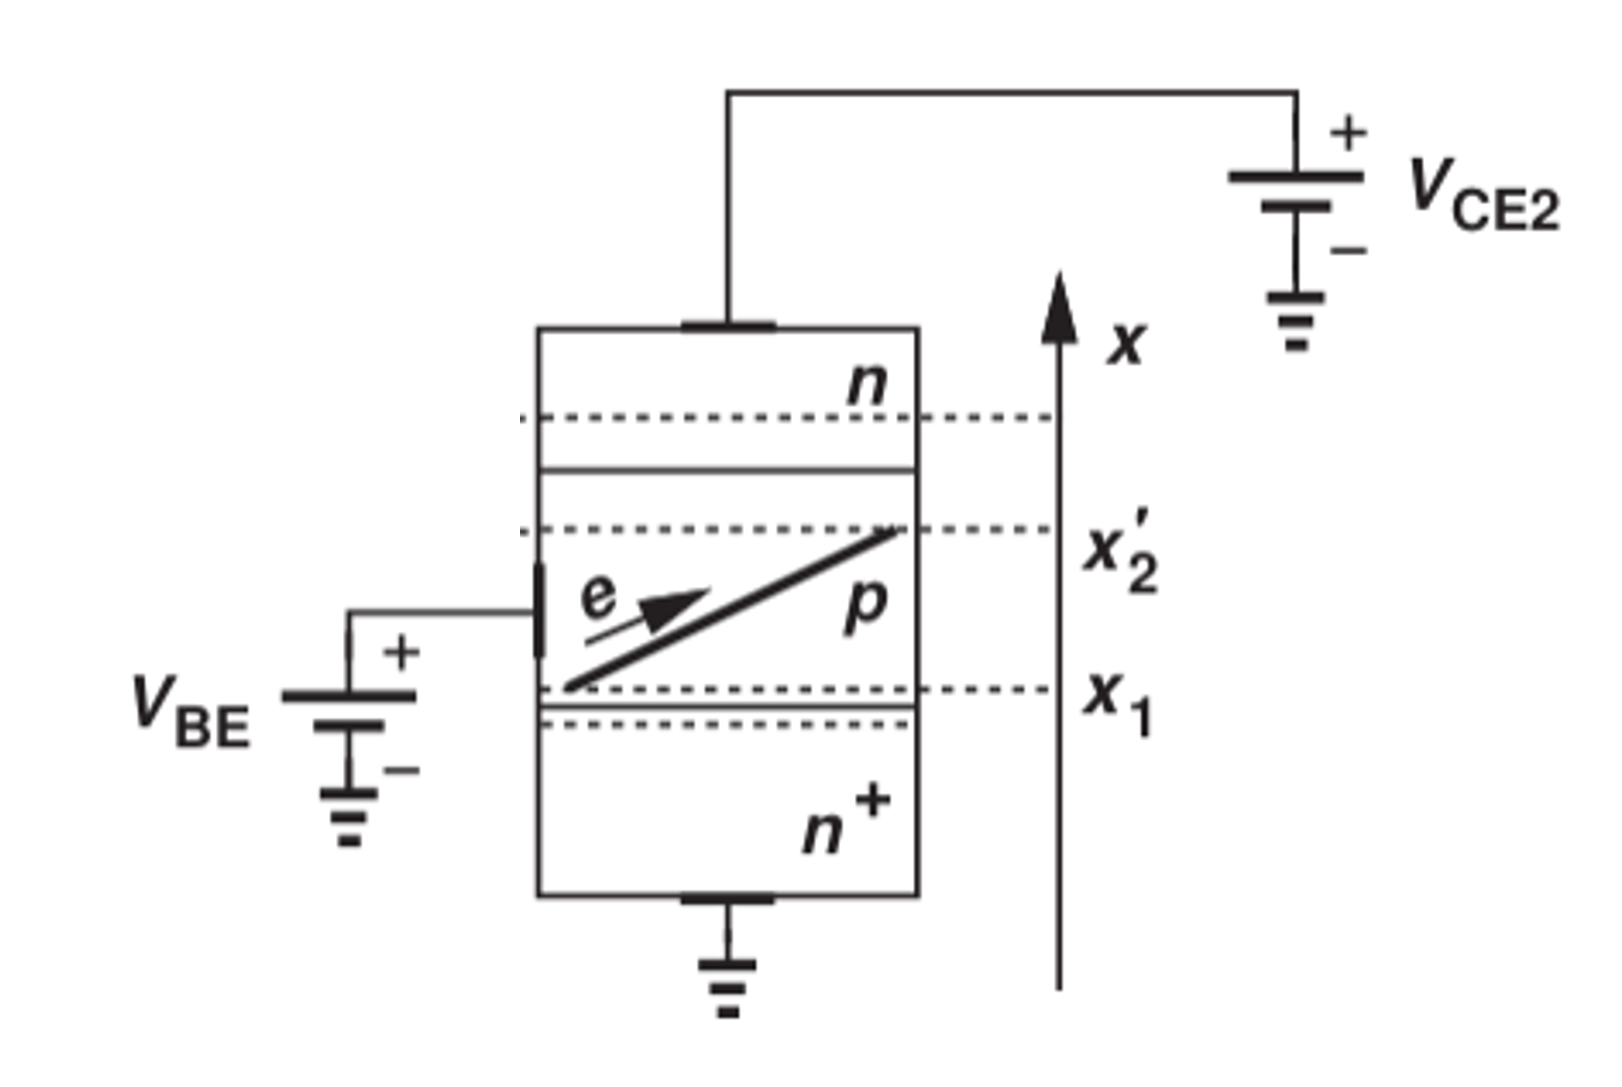
\includegraphics[width=\textwidth]{figuras/efecto_early_sentido_fisico_2.png}
\end{figure}

El parámetro $V_A$ es la tensión de Early. Este parámetro depende de la tecnología.

\end{column}
\begin{column}{0.6\textwidth}

\begin{itemize}
    \item Como la base es más angosta, la corriente aumenta.
    \item Para modelar este efecto, se asume que el ancho de la base es ``constante'' y se agrega un factor de corrección, que se interpreta como un porcentaje:
    \[ I_C = \dfrac{A_E q D_n n_i^2 }{N_E W_B} \left( e^{V_{BE}/V_t} - 1 \right) \left( 1 + \dfrac{V_{CE}}{V_A} \right) \]
    \[ I_C = I_S \left( e^{V_{BE}/V_t} - 1 \right) \left( 1 + \dfrac{V_{CE}}{V_A} \right) \]
\end{itemize}

\end{column}
\end{columns}

\end{frame}


\begin{frame}{Curvas características con efecto Early}

\begin{figure}[H]
    \centering
    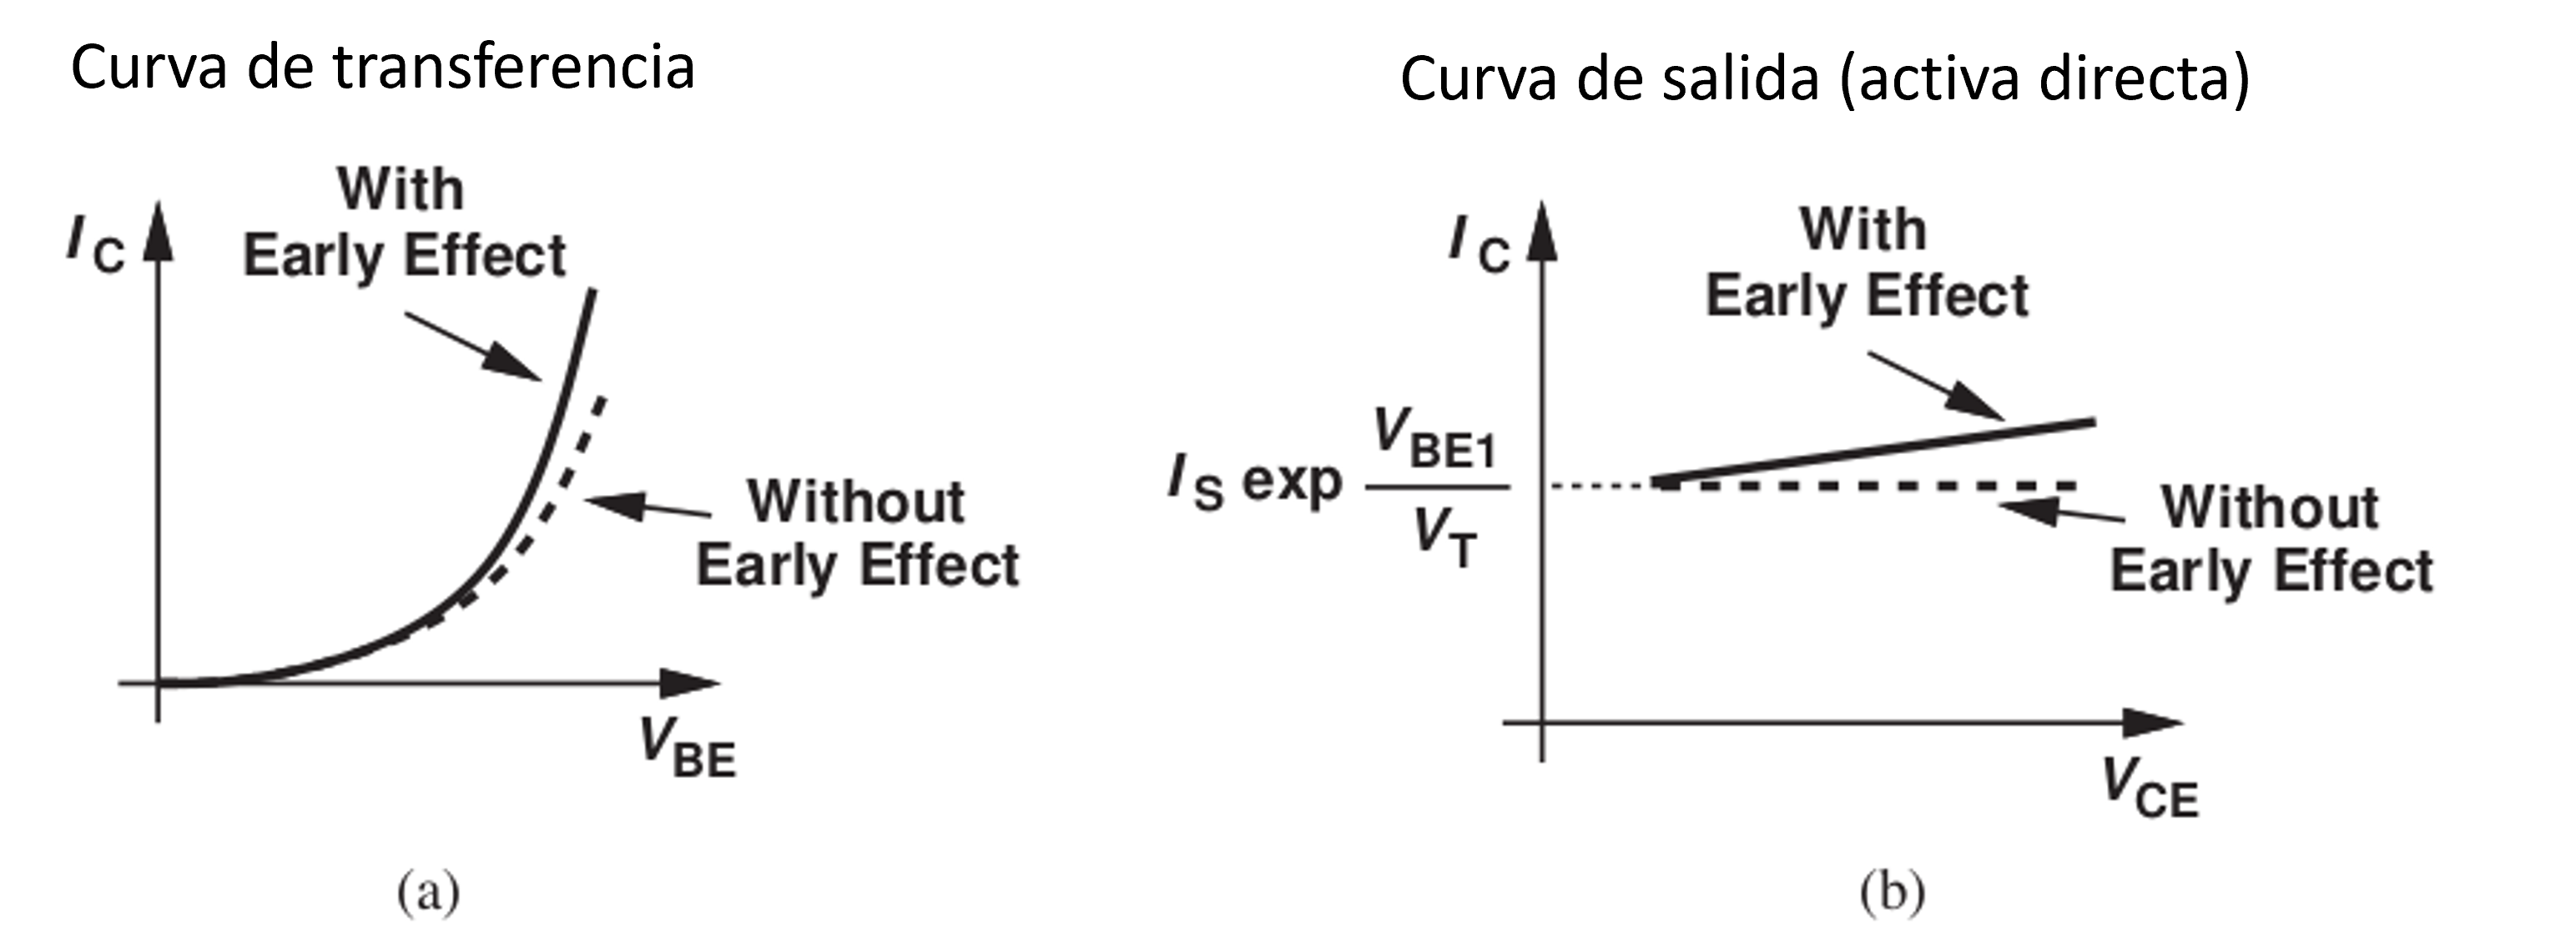
\includegraphics[width=\textwidth]{figuras/efecto_early_curvas.png}
\end{figure}

\begin{itemize}
    \item En ambas curvas se observa un incremento en la corriente de colector.
    \item \textbf{El transistor en Activa Directa ya no es una fuente de corriente ideal.}
\end{itemize}
    
\end{frame}


\begin{frame}{Impedancia de salida}

La pendiente de la curva de salida indica que $I_C$ ya no es constante con $V_{CE}$.

\begin{columns}
\begin{column}{0.5\textwidth}

\begin{figure}[H]
    \centering
    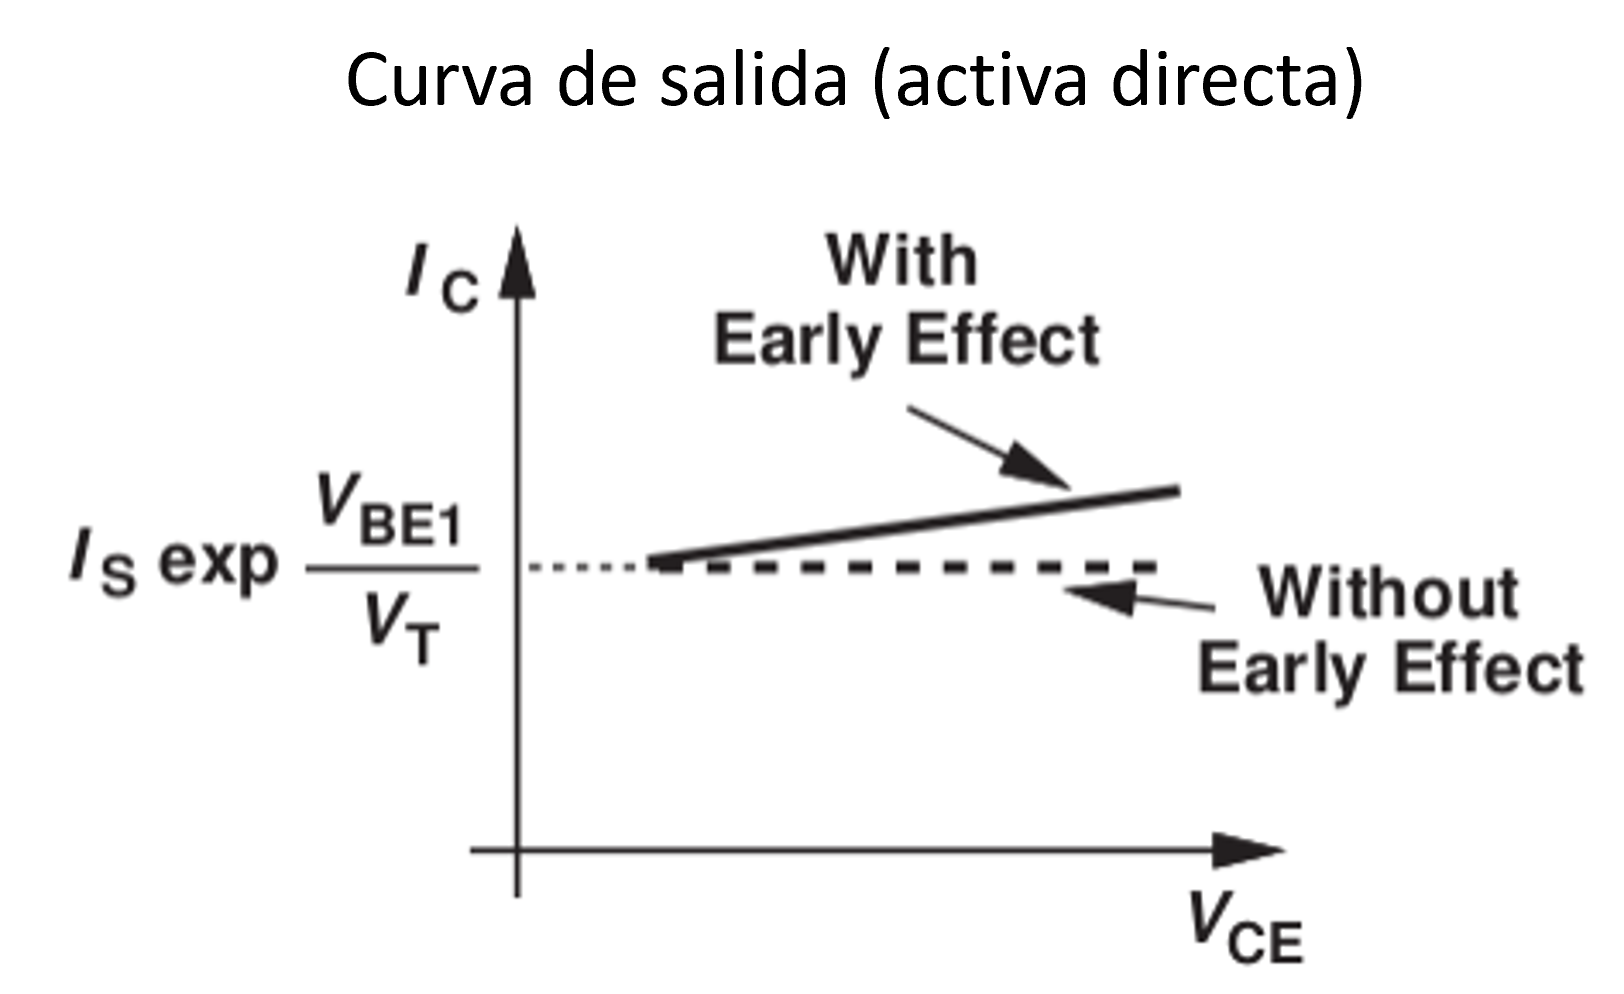
\includegraphics[width=\textwidth]{figuras/curva_salida_con_early.png}
\end{figure}

\end{column}
\begin{column}{0.5\textwidth}

La pendiente de esta curva es:
%
\[ \dfrac{\partial I_C}{\partial V_{CE} } = I_S \left( e^{V_{BE}/V_t} \right) \left( \dfrac{1}{V_A} \right)  \]
%
\[ \dfrac{\partial I_C}{\partial V_{CE} } = \dfrac{I_C}{V_A} \]

\vspace{5mm}
Se define la resistencia de salida:
%
\[ r_o = \dfrac{V_A}{I_C} \]

\end{column}
\end{columns}
    
\end{frame}


\begin{frame}{Ejemplo 1: Polarización sin efecto Early vs. con efecto Early}

Un transistor bipolar NPN tiene una corriente de colector de 1 mA con $V_{CE} = 2\ V$. Determine la tensión $V_{BE}$ requerida si $V_A = \infty$ o si $V_A = 20\ V$. 

Asuma $I_S = 2\times{}10^{-16}\ A$.


\begin{columns}
\begin{column}{0.5\textwidth}

\centering
\textbf{Sin efecto Early}
\[ V_{BE} = V_t \ln \left(\dfrac{I_C}{I_S}\right) \]
\[ V_{BE} = 26\ mV \ln \left(\dfrac{1\ mA}{2\times{}10^{-16}\ A}\right) \]
\[ V_{BE} = 760.3\ mV \]

\end{column}
\begin{column}{0.5\textwidth}

\centering
\textbf{Con efecto Early}
\[ V_{BE} = V_t \ln \left( \dfrac{I_C}{I_S} \cdot \dfrac{1}{1 + \dfrac{V_{CE}}{V_A}} \right) \]
\[ V_{BE} = 757.8\ mV \]

\end{column}
\end{columns}

\vspace{5mm}
La tensión requerida es menor con efecto Early.
\end{frame}


\begin{frame}{Ejemplo 2: Polarización PNP con efecto Early}

Determine el punto de operación para cada uno de los circuitos mostrados en la figura. Asuma las siguientes constantes para todos los transistores: $I_S = 3\times{}10^{-17}\ A$, $\beta=100$, $V_A = 1\ V$.

\begin{figure}
    \centering
    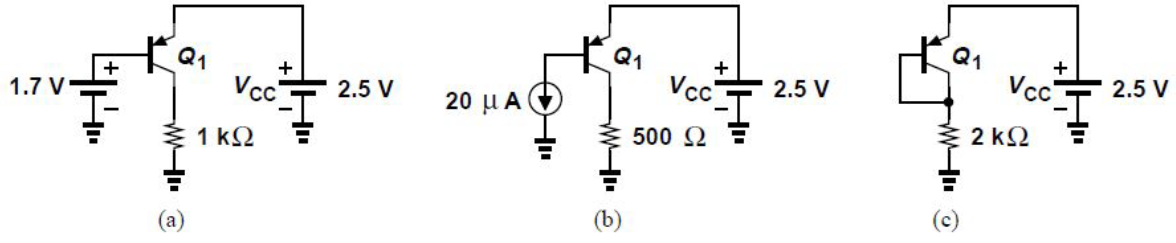
\includegraphics[width=\textwidth]{figuras/efecto_early_ejemplo_2.png}
\end{figure}
    
\end{frame}


\begin{frame}{Solución 2: Polarización PNP con efecto Early (a)}

\begin{figure}
    \flushleft
    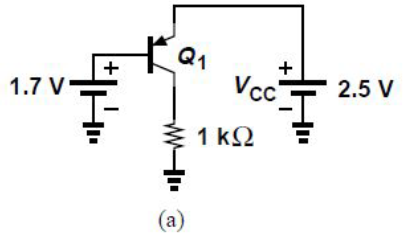
\includegraphics[width=0.4\textwidth]{figuras/efecto_early_ejemplo_2_a.png}
\end{figure}
    
\end{frame}


\begin{frame}{Solución 2: Polarización PNP con efecto Early (b)}

\begin{figure}
    \flushleft
    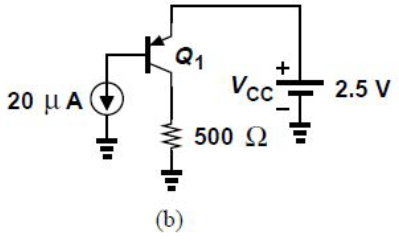
\includegraphics[width=0.4\textwidth]{figuras/efecto_early_ejemplo_2_b.png}
\end{figure}
    
\end{frame}


\begin{frame}{Solución 2: Polarización PNP con efecto Early (c)}

\begin{figure}
    \flushleft
    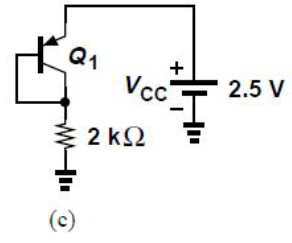
\includegraphics[width=0.3\textwidth]{figuras/efecto_early_ejemplo_2_c.png}
\end{figure}
    
\end{frame}


\begin{frame}{Ejemplo 3: Polarización NPN con degeneración y efecto Early}

Determine la corriente del circuito mostrado con los siguientes modelos:

\begin{enumerate}
    \item Modelo de tensión constante $V_{BE} = 0.7\ V$, $\beta = 100$.
    \item Modelo exponencial $I_S = 6\times{}10^{-16}\ A$ sin efecto Early $V_A = \infty$, $\beta = 100$.
    \item Modelo exponencial $I_S = 6\times{}10^{-16}\ A$ con efecto Early, $V_A = 5\ V$, $\beta = 100$.
\end{enumerate}

\begin{figure}[H]
    \centering
    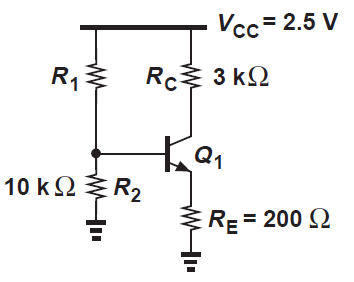
\includegraphics[width=6cm]{figuras/efecto_early_ejemplo_3.png}
\end{figure}
    
\end{frame}


\begin{frame}{Solución 3: Polarización NPN con degeneración y efecto Early (a)}

\begin{columns}
\begin{column}{0.35\textwidth}

\begin{figure}[H]
    \flushleft
    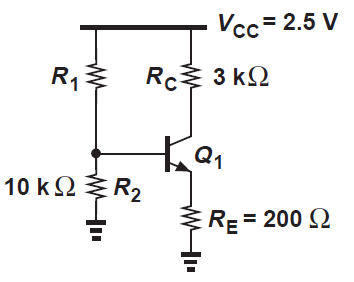
\includegraphics[width=\textwidth]{figuras/efecto_early_ejemplo_3.png}
\end{figure}

\end{column}
\begin{column}{0.65\textwidth}

\textbf{Modelo de tensión constante}

\end{column}
\end{columns}
    
\end{frame}


\begin{frame}{Solución 3: Polarización NPN con degeneración y efecto Early (b)}

\begin{columns}
\begin{column}{0.35\textwidth}

\begin{figure}[H]
    \flushleft
    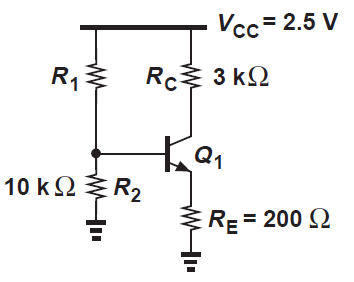
\includegraphics[width=\textwidth]{figuras/efecto_early_ejemplo_3.png}
\end{figure}

\end{column}
\begin{column}{0.65\textwidth}

\textbf{Modelo exponencial sin efecto Early}

\end{column}
\end{columns}
    
\end{frame}


\begin{frame}{Solución 3: Polarización NPN con degeneración y efecto Early (c)}

\begin{columns}
\begin{column}{0.35\textwidth}

\begin{figure}[H]
    \flushleft
    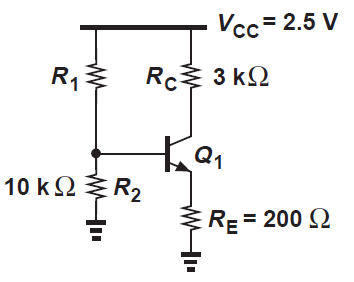
\includegraphics[width=\textwidth]{figuras/efecto_early_ejemplo_3.png}
\end{figure}

\end{column}
\begin{column}{0.65\textwidth}

\textbf{Modelo exponencial con efecto Early}

\end{column}
\end{columns}
    
\end{frame}


\begin{frame}{Lecturas recomendadas}

\begin{itemize}
    \item Razavi, B. (2013). Fundamentals of Microelectronics, 2nd edition. Chapter 4: Physics of Bipolar Transistors, pp. 144-150, Wiley, Los Angeles, California.
\end{itemize}

\end{frame}

\end{document}
